\subsection[ROS2 Integration]{ROS2 Integration \myAuthor{Sami Hamza}}
\subsubsection{Aufgaben}
Die wesentliche Aufgabe der ROS2 Implementierung ist das Empfangen der von Team Digitalize segmentierten Bilder der Puzzleteile. Anschließend muss das Puzzle anhand der empfangen Bilder gelöst werden. Danach soll das Puzzle im Visualizer aufgebaut werden. Hierfür muss für je ein Puzzleteil die Übergabeposition für den Roboter und die Zielposition im Robotersystem berechnet werden. Die Start und Endpositionen werden dann über das Topic ``solver/nextpiece'' an die Control-Node versendet. Zusätzlich muss die Visualizer-Node über das Topic ``solver/startpos'' die Startposition des aktuellen Teils erhalten. Wird das Puzzleteil abgelegt, so erhält die Solver-Node diese Information über das Topic ``control/puzzlebool'' und soll die Informationen für das nächste Teil versenden. 

\subsubsection{Schnittstellen}
\autoref{fig:topics} gibt eine Übersicht über die verwendeten Schnittstellen aus Sicht der Solver-Node.

\begin{figure}[H]
    \centering
    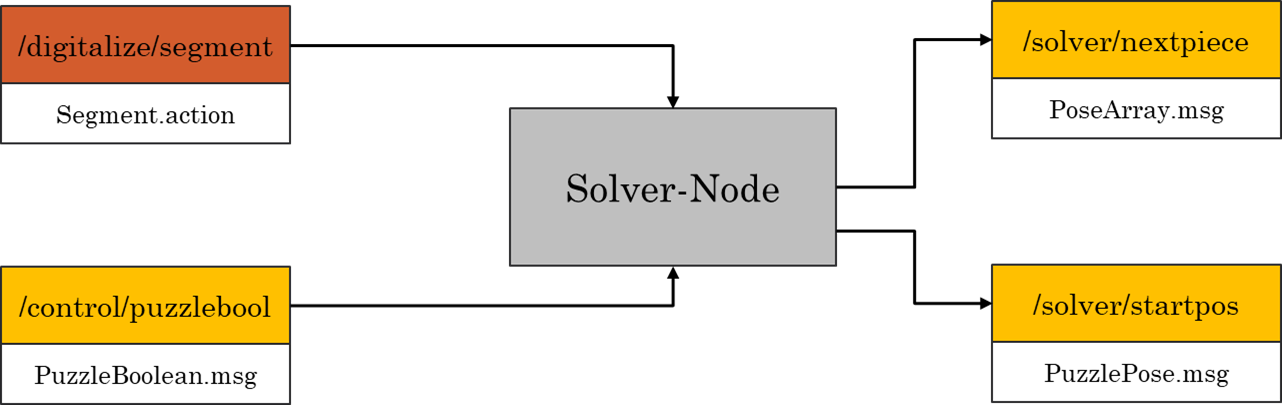
\includegraphics[width=0.8\textwidth]{sections/solver/images/topics.png}
    \caption{ROS2-Schnittstellen Übersicht.}
    \label{fig:topics}
\end{figure}

\paragraph{Solver - Digitalize} Hier wird als Art der Kommunikation die von ROS2 bereitgestellte Action-Server Schnittstelle verwendet. Der Server kann über das Topic ``/digitalize/segment'' erreicht werden. Diese erlaubt es Clients (hier die Solver-Node) über eine Goal-Anfrage einen den Mechanismus in der Server-Node (hier die Digitalize-Node) zu aktivieren. Rückmeldung zum Status der Abfrage kann Client-seitig über die \textit{goal\_response\_callback} verarbeitet werden. Wird die Anfrage angenommen, führt der Server den Benutzer definierten Ablauf durch und sendet währenddessen Feedback-Nachrichten, welche hier von der \textit{feedback\_callback} abgefangen werden können und für den Bildtransport verwendet werden. Abschließend wird eine Result-Nachricht versendet, welche von der \textit{get\_result\_callback} abgefangen wird und dem Client das Ende des Ablaufs indiziert. Diese Struktur ist ideal für den Transport der segmentierten Bilder, da diese sicherstellt, dass beide Parteien für die Kommunikation bereit sind. Außerdem muss die Solver-Node keine Kenntnis darüber haben, wie viele Bilder gesendet werden, da das Ende der Übertragung eindeutig gekennzeichnet wird. 

\paragraph{Solver - Visualize}
Über diese Schnittstelle teilt die Solver-Nodel der Visualizer-Node die Startposition (Spawn-Punkt) der Puzzleteile mit. Es handelt sich hierbei Solver-seitig um einen einfachen Publisher, der Nachrichten vom eigens definiertem Typen \textit{PuzzlePose} auf das Topic ``solver/startpos'' published. \autoref{lst:puzzlepose} zeigt die Definition der versendeten Nachricht. Diese beinhaltet die jeweilige Piece-ID des Puzzleteils und die Posen Information, welche durch eine Position als \textit{Point} und eine Orientierung als \textit{Quaternion} im Robotersystem (Einheit Meter) definiert ist.
\begin{lstlisting}[language=Python, caption={Nachrichten Definition für     PuzzlePose.msg},label=lst:puzzlepose]
# id of the puzzle piece
int32 id
# pose of the puzzle piece (with x- and y-axis aligned 
# with image x- and y-axis) in robot base frame
geometry_msgs/Pose pose 

\end{lstlisting}

\paragraph{Solver - Control}
Die Solver-Node übermittelt der Control-Node mit dieser Schnittstelle die Startposition (Spawn-Punkt) und die Zielposition der Puzzleteile. Es handelt sich hierbei Solver-seitig wieder um einen einfachen Publisher, der Nachrichten des in geometry\_msgs von ROS vordefinierten Nachrichtentyps  \textit{PoseArray} auf das Topic ``solver/startpos'' published. Diese Nachricht enthält ein Array aus ROS-Poses, welche durch eine Position und eine Orientierung als Quaternion im Robotersystem (Einheit Meter) definiert sind.
 
\subsubsection{Node - Ablauf}
Um die gesamten Aufgaben zu erfüllen wird im Rahmen des Projektes ein monolithischer Ansatz gewählt. Dieser bietet sich an, da alle Aufgaben sukzessiv gelöst werden können und damit sehr schön durch Callback-Funktionen realisiert werden kann. In \autoref{fig:sequence} ist der sequenzielle Ablauf der Solver Node-Callbacks dargestellt. 
\begin{enumerate}
    \item Der `main-Thread'' main-Node initiert den Ablauf über die \textit{send\_segment\_goal}-Funktion und dient als warte-Thread falls grade keine Callback aktiv ist. Sie sendet zu Beginn eine Anfrage an den Digitalize-Action-Server (Event $E_1$). 
    \item Die Antwort der Action-Server-Goal-Anfrage wird empfangen (Event $E_2$) und anschließend in der \textit{goal\_response\_callback}-Funktion verarbeitet.
    \item Dannach wird auf Feedback-Nachrichten, die die Bilder enthalten, gewartet. Wird eine dieser Nachrichten empfangen (Event $E_3$), so wird das Bild ausgelesen und unter dem Namen ``image\_$<$pid$>$\_.png'' abgespeichert. Dabei ist pid, die mit dem Image versandte Piece-ID.
    \item Wurden alle Bilder gesendet, sendet der Server die Result-Nachricht und die \textit{get\_result\_callback}-Funktion wird aufgerufen. In dieser wird das Puzzle gelöst. In Folge dessen wird das erste Teil aus der Solver Historie gezogen und dafür die Start- und Endposition berechnet. Hierbei muss die Konversion zwischen Posen in Pixelkoordinaten, wie sie im gelösten Puzzle verwendet werden, und Metern ((Faktor 0,00004 mm/pixel)) für das Control-Team bzw. Milimetern (Faktor 0,04 mm/pixel) für das Visualizer-Team beachtet werden. Die korrespondierenden Posen werden in die Topics ``solver/nextpiece'' und ``solver/startpos'' gepublished.
    \item Sobald der Solver eine PuzzleBool-Message auf dem Topic ``control/puzzlebool'' erhält (Event $E_4$) wird in der \textit{puzzle\_bool\_callback}-Funktion überprüft ob ein Wechsel von True auf False stattgefunden hat, was dem Ablegen des Teils an der Zielposition entspricht. Ist dies der Fall, so wird das nächste Teil aus der Solver Historie gezogen, die Posen berechnet und die Nachrichten gepublished (Analog zur \textit{get\_result\_callback}-Funktion). Wurden bereits alle Teile aus der Solver-Historie gezogen, so wird die Node nach erneuten Aufrufen der \textit{puzzle\_bool\_callback}-Funktion beendet.
\end{enumerate}
     
\begin{figure}[H]
    \centering
    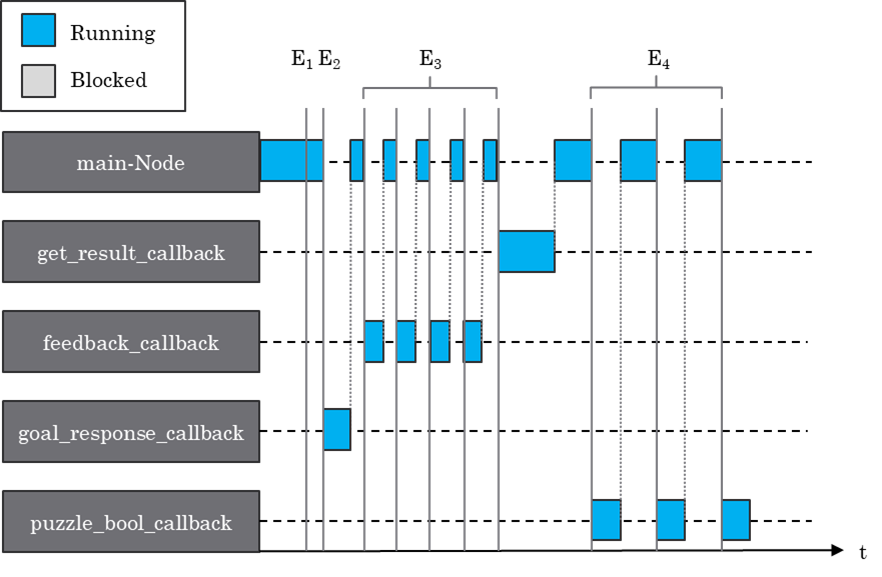
\includegraphics{sections/solver/images/sequence_example.png}
    \caption{Sequenzbeispiel zur Veranschaulichung der Callback-Interaktion.}
    \label{fig:sequence}
\end{figure}

\subsubsection{Schnittstellentests}
Im Rahmen des Projekts wurden jeweils in Zusammenarbeit mit den anderen Teams Integrationstests durchgeführt. Hierfür wurden Teilfunktionalitäten manuell durch Starten der betroffenen Nodes über ROS-Launchfiles auf Richtigkeit überprüft.

\subsubsection{Fazit}
Im Allgemeinen lässt sich sagen, dass die Funktionalität gut gewährleistet ist. Allerdings könnte der entwickelte Code durch Refaktoring noch besser strukturiert werden. Auch die gewählten Schnittstellen weisen noch viel Verbesserungspotential auf. So könnte man anstatt der für den Action-Server verwendeten \textit{sensor\_msgs/Image} Feedback-Nachricht eine \textit{sensor\_msgs/CompressedImage} Feedback-Nachricht verwenden, um effizienter zu Transportieren. Ein weiterer Problematischer Aspekt ist, dass die Feedbacknachrichten nicht zu schnell aufeinander folgen dürfen, da sonst Bilder Solver-seitig verloren gehen. Das Problem kann Digitalize-seitig durch eine ausreichend lange Verzögerung gelöst werden. Der Begriff ausreichend ist aber start Abhäng von den zu Verfügung stehenden System-Resourcen. Auch Redundanzen bezüglich der Startposition könnten reduziert werden, indem sowohl der Visualizer, als auch die Control Node auf das ``solver/nextpiece'' Topic subscriben würden. Denn in dieser Nachricht ist die Startposition ja ebenfalls enthalten. Auch unnötige Konvertierungen der Einheiten könnten durch einheitlich Konventionen gespart werden.